\documentclass[problem]{mcs}

\begin{pcomments}
  \pcomment{CP_coin_flips}
  \pcomment{from: S09.cp12r}
\end{pcomments}

\pkeywords{
  probability
}

%%%%%%%%%%%%%%%%%%%%%%%%%%%%%%%%%%%%%%%%%%%%%%%%%%%%%%%%%%%%%%%%%%%%%
% Problem starts here
%%%%%%%%%%%%%%%%%%%%%%%%%%%%%%%%%%%%%%%%%%%%%%%%%%%%%%%%%%%%%%%%%%%%%

% F09, S09

\begin{problem}
  To determine which of two people gets a prize, a coin is flipped twice.
  If the flips are a Head and then a Tail, the first player wins.  If the
  flips are a Tail and then a Head, the second player wins.  However, if
  both coins land the same way, the flips don't count and whole the
  process starts over.

  Assume that on each flip, a Head comes up with probability $p$,
  regardless of what happened on other flips.  Use the four step method to
  find a simple formula for the probability that the first player wins.
  What is the probability that neither player wins?

  Suggestions: The tree diagram and sample space are infinite, so you're
  not going to finish drawing the tree.  Try drawing only enough to see a
  pattern.  Summing all the winning outcome probabilities directly is
  difficult.  However, a neat trick solves this problem and many others.
  Let $s$ be the sum of all winning outcome probabilities in the whole
  tree.  Notice that {\em you can write the sum of all the winning
    probabilities in certain subtrees as a function of $s$}.  Use this
  observation to write an equation in $s$ and then solve.

\begin{solution}
In the tree diagram below, the small triangles represent
subtrees that are themselves complete copies of the whole tree.

\bigskip
\centerline{\resizebox{!}{3in}{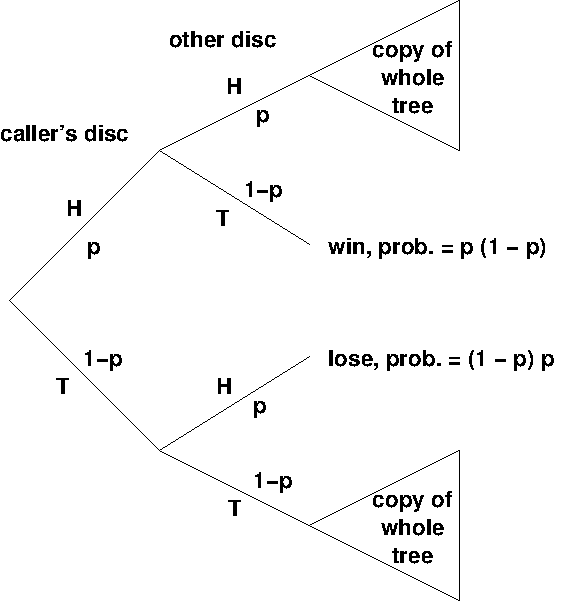
\includegraphics{fair-frisbee}}}
\bigskip

Let $s$ equal the sum of all winning probabilities in the whole tree.
There are two extra edges with probability $p$ on the path to each
outcome in the top subtree.  Therefore, the sum of winning
probabilities in the upper tree is $p^2 s$.  Similarly, the sum of
winning probabilities in the lower subtree is $(1-p)^2 s$.  This gives
the equation:

\begin{equation*}
s = p^2 s + (1-p)^2 s + p (1-p)
\end{equation*}

The solution to this equation is $s = 1/2$, for all $p$ between 0 and
1.

By symmetry, the probability that the first player loses is 1/2.  This
means that the event, if any, of flipping forever can only have
probability zero.

Formally, the sample space is the (infinite) set of leaves of the tree,
namely,
\[
\sspace \eqdef \set{\mathtt{TT,HH}}^*\cdot \set{\mathtt{HT,TH}}
\]
where $\set{\mathtt{TT,HH}}^*$ denotes the set of strings formed by
concatenating a sequence of \texttt{HH}'s and \texttt{TT}'s.  For example,
\[
\mathtt{TTTTHHHT, HHTTTH, HHHHHHHHHT, HT} \in \sspace.
\]
For any string $s \in \sspace$,
\[
\pr{s} \eqdef p^{\text{\#\texttt{H}'s in $s$}}(1-p)^{\text{\#\texttt{T}'s in $s$}}.
\]
To verify that is defines a probability space, we must show that
$\sum_{s \in \sspace} \pr{s} = 1$:

\begin{align*}
\sum_{s \in \sspace} \pr{s}
   & = \sum_{n \geq 0} \sum_{s \in \sspace, \lnth{s} =2n+2}
            p^{\text{\#\texttt{H}'s in $s$}}(1-p)^{\text{\#\texttt{T}'s in $s$}}\\
   & = \sum_{n \geq 0} \sum_{i+j=n} p^{2i}(1-p)^{2j}p(1-p) 
          & \text{(strings that end in \texttt{HT})}\\
   &    \quad + \sum_{n \geq 0} \sum_{i+j=n} p^{2i}(1-p)^{2j}p(1-p)
          & \text{(strings that end in \texttt{TH})}\\
   & = 2p(1-p)\sum_{n \in \naturals} \paren{p^2+(1-p)^2}^n\\
   & = \frac{2p(1-p)}{1- (p^2+(1-p)^2)}\\
   & = \frac{2p(1-p)}{2p^2 +2p} = 1.
\end{align*}
\end{solution}
\end{problem}


%%%%%%%%%%%%%%%%%%%%%%%%%%%%%%%%%%%%%%%%%%%%%%%%%%%%%%%%%%%%%%%%%%%%%
% Problem ends here
%%%%%%%%%%%%%%%%%%%%%%%%%%%%%%%%%%%%%%%%%%%%%%%%%%%%%%%%%%%%%%%%%%%%%

\endinput
